\documentclass{article}

\usepackage[margin=1in]{geometry}
\usepackage{amsmath,amsthm,amssymb}
\usepackage{bbm,enumerate,mathtools}
\usepackage[hidelinks]{hyperref}
\usepackage{tikz}
\usetikzlibrary{arrows}

\newcommand{\fn}[3]{#1 \colon #2 \rightarrow #3}
\newcommand{\set}[1]{\left\{#1\right\}}
\newcommand{\pd}[2]{\frac{\partial #1}{\partial #2}}

\theoremstyle{definition}
\newtheorem{definition}{Definition}[section]

% \theoremstyle{example}
\newtheorem{example}{Example}[section]

% \theoremstyle{conjecture}
\newtheorem{conjecture}{Conjecture}[section]

\theoremstyle{remark}
\newtheorem{remark}{Note}[section]

\newtheorem{theorem}{Theorem}[section]

\begin{document}

\title{Geodesics}
\author{Peter Kagey}

\maketitle
% How do we measure the length of a curve?

% Definition of geodesic
\begin{section}{Preliminaries}
  The running intuition in this paper is to think of a creature who lives in the
  manifold walking in a ``straight'' line in some sense at a constant
  (nonzero) speed--in other words, the creature isn't accelerating.

  In the case where $\mathbb R^n$, the notion of acceleration along a path at
  some point in time is easy to naively define, since the notion of adding
  velocity vectors at two different points along the curve can be done naively,
  and so the second derivative works in the typical sense \[
    \gamma''(t) = \lim_{h \rightarrow 0} \frac{\gamma'(t + h) - \gamma'(t)}{h}.
  \] However, one has to be much more careful when talking about acceleration
  in a general manifold. In particular, $T_{\gamma(t)}$ and $T_{\gamma(t+h)}$ are
  generally different tangent spaces, and the notion of adding their vectors is
  decidedly more subtle. In particular, if a manifold is isometrically embedded
  into Euclidean space via $\fn f M {\mathbb R^n}$, the velocity along the image
  of a curve is preserved, but the acceleration is not quite the same---instead,
  the acceleration in $M$ corresponds to the acceleration in $f(M)$
  of the projection of the acceleration to the tangent plane.
  However, capturing this notion intrinsically is more subtle.
  % Note: geodesics satisfy the properties of (non-euclidean) geometry
  % In this section, $M$ will always refer to a connected smooth manifold with or
  % without boundary unless otherwise noted, and $\nabla$ will refer to a connection in
  % $TM$.


  \begin{definition}[Connection]
    Let $\fn \pi E M$ be a smooth vector bundle over $M$. Then a connection in
    $E$ is any map that sends a tangent vector field and a section of $E$ to
    another section of $E$ \[
      \fn{\nabla}{\mathfrak X(M) \times \Gamma(E)}{\Gamma(E)}
    \] denoted $\nabla_XY := \nabla(X, Y)$ and satisfying the following three properties:
    \begin{enumerate}[(i)]
      \item $\displaystyle\nabla_{f_1X_1 + f_2X_2}Y = f_1\nabla_{X_1}Y + f_2\nabla_{X_2}Y$,
      \item $\displaystyle\nabla_X(a_1Y_1 + a_2Y_2) = a_1\nabla_X Y_1 + a_2\nabla_XY_2$, and
      \item $\displaystyle\nabla_X(fY) = f\nabla_{X}Y + \underbrace{(Xf)}_{\in C^\infty(M)}Y$.
    \end{enumerate}
    Connections are generalizations of directional derivatives with respect to
    $X$, a tangent vector field.
  \end{definition}
  \begin{remark} % https://youtu.be/nEaiZBbCVtI
    In the case where $\Gamma(E) = C^\infty(M)$, $\nabla(X, f) := Xf$ satisfies
    the above properties. In particular, $\nabla$ can be thought of as a
    prescription for extending $\fn X {C^\infty(M)}{C^\infty(M)}$ to act on other
    vector bundles.
  \end{remark}
  \begin{example}
    Consider the case of $M = \mathbb R^3$ with the section of the tangent
    bundle given by  $(x, 1, e^y) = X \in \mathfrak X(\mathbb R^3)$
    and the rank 2 vector bundle $(x^2, y + z) = Y \in \Gamma(E)$. Then taking
    the derivative of $Y$ along $X$ yields \[
      \nabla_XY = \underbrace{\begin{bmatrix}
        \displaystyle\pd{x^2}{x} & \displaystyle\pd{x^2}{y} & \displaystyle\pd{x^2}{z} \\
        \\
        \displaystyle\pd{(y+z)}{x} & \displaystyle\pd{(y + z)}{y} & \displaystyle\pd{(y + z)}{z}
      \end{bmatrix}}_{dY(x,y,z)}
      \underbrace{\begin{bmatrix}
        x \\~\\ 1 \\~\\ e^y
      \end{bmatrix}}_{X} =
      \begin{bmatrix}
        2x^2 \\~\\ 1 + e^y
      \end{bmatrix}.
    \] The matrix multiplication perspective makes it clearer to see that in
    this case (i) $\nabla$ is $C^\infty(\mathbb R^3)$-linear in the first
    term, because the column vector is $C^\infty(\mathbb R^3)$-linear,
    (ii) $\nabla$ is $\mathbb R$-linear in the second term because both partial
    derivatives and matrices are $\mathbb R$-linear, and (iii) holds by doing
    the product rule entrywise in the Jacobian matrix $d(fY)(x,y,z)$.
  \end{example}
  These conditions capture, in some sense, the ``essential qualities'' of
  taking the directional derivative of a vector bundle over a given section of
  the tangent bundle.

  % Being able to take the derivative of a section of a vector bundle in the
  % direction of the tangent bundle is the first step to being able to take the
  \begin{definition}[Covariant derivative along a curve]
    Let $\nabla$ be a connection in tangent bundle $TM$, and let $\gamma$ be a
    curve in $M$. Then the \textbf{covariant derivative along} $\boldsymbol{\gamma}$ is the
    (unique) map \[
      \fn {D_\gamma }{\mathfrak X(\gamma)}{\mathfrak X(\gamma)}
    \] satisfying the following three properties \begin{enumerate}[(i)]
      \item $\displaystyle D_\gamma (aV + bW) = aD_\gamma V + bD_\gamma W$
      \item $\displaystyle D_\gamma (fV) = f'V + fD_\gamma V$
      \item $\displaystyle D_\gamma V(t) = \nabla_{\gamma'(t)}\widetilde{V}$ for every extension $\widetilde V$ of $V$.
    \end{enumerate}
  \end{definition}
  \begin{remark}
    This definition is sensible, because (i) and (ii) correspond to (ii) and
    (iii) in the definition of a connection, and the last condition is roughly
    equivalent to (i) in the definition of a connection: that is, the covariant
    derivative is $C^\infty(M)$-linear in the first component, so it only
    depends on the vector field pointwise.
  \end{remark}

  % \begin{remark}
    When on a Riemannian manifold, it is common to use a particular connection
    called the Levi-Civita connection, which is compatible with the metric in
    the expected way, and which has some other nice properties.
  % \end{remark}
  \begin{definition}[Levi-Civita connection]
    The \textbf{Levi-Civita connection} is a connection $\nabla$ such that
    \begin{enumerate}[(a)]
      \item the metric is preserved under $\nabla$, that is, $\nabla_{\!(-)\,}g \equiv 0$, and
      \item for any vector fields $X, Y \in \mathfrak(M)$, $\nabla_XY - \nabla_YX = [X, Y]$.
    \end{enumerate}
  \end{definition}
  \begin{remark}
    When the Levi-Civita connection exists, it is unique.
  \end{remark}
  \begin{remark}
    A connection that satisfies the second condition in the definition of the
    Levi-Civita connection is called``torsion-free'', because the torsion is
    defined as \[
      T(X, Y):= \nabla_XY - \nabla_YX - [X, Y].
    \]
    % What is torsion on a 2-manifold? Always 0?
  %   The inner product $g$ on the tangent bundle is a vector space, and
  %   so the action of $\nabla$ on $g$ is well-defined.
  \end{remark}
  \begin{definition}[Acceleration of a curve]
   For every smooth map from an interval to the manifold, $\fn \gamma I M$,
   define the \textbf{acceleration of $\gamma$} as the vector field
   $D_\gamma  \gamma'$ along $\gamma$.
  \end{definition}

  \begin{definition}[Geodesic]
    A smooth curve $\gamma$ is called a \textbf{geodesic} (with respect to
    $\nabla$) if it's acceleration is zero: $D_\gamma \gamma' \equiv 0$.
  \end{definition}

  % \begin{figure}
  %   \begin{tikzpicture}
  %   % Example of a geodesic or two.
  %   % Poincare disk?
  %   \end{tikzpicture}
  % \end{figure}

  \begin{theorem}[Existence and uniqueness for geodesics] % Lee Theorem 4.27
    Let $M$ be a smooth manifold and $\nabla$ a connection. Then for every
    $p \in M$, $v \in T_pM$ and $t_0 \in \mathbb R$, there exists an open
    interval $I \subset \mathbb R$ containing $t_0$ and a geodesic
    $\fn \gamma I M$ satisfying $\gamma(t_0) = p$ and $\gamma'(t_0) = v$.

    Furthermore, any two geodesics with the same initial conditions agree on
    their common domain.
  \end{theorem}
  \begin{proof}[Proof idea]
    This result follows from moving to local coordinates in a way that respects
    the connection, and then making an appeal to uniqueness and existence for
    (second order) ordinary differential equations.
  \end{proof}

  \begin{definition}[Geodesic extension]
    Given a geodesic $\fn \gamma I M$, an \textbf{extension of} $\boldsymbol{\gamma}$ is a map
    $\fn {\widetilde \gamma} {\widetilde I} M$ such that \begin{enumerate}[(i)]
      \item $I$ is a subset of $\widetilde I$,
      \item the map $\widetilde \gamma$ is itself a geodesic, that is $D_{\widetilde\gamma}{\widetilde\gamma'} \equiv 0$, and
      \item the map agrees on the original interval, that is $\widetilde \gamma|_I = \gamma$.
    \end{enumerate}
  \end{definition}
  \begin{remark}
    A \textit{proper} extension is an extension in which condition (i) is strengthened
    such that $I$ is a \textit{proper} subset of $\widetilde I$.
  \end{remark}
  \begin{remark}
    A geodesic with no proper extension is called a \textbf{maximal} geodesic.
  \end{remark}
  \begin{definition}[Geodesically complete manifold]
    A manifold is called geodesically complete (with respect to $\nabla$) if
    every geodesic curve $\gamma$ has an ``all-time'' extension to
    $\fn {\widetilde\gamma} {\mathbb R} {M}$.
  \end{definition}
  \begin{definition}[Closed geodesic]
    A geodesic $\fn \gamma I M$ is called \textbf{closed} if there exist
    two points $t_1 \neq t_2 \in I$ such that $\gamma(t_1) = \gamma(t_2)$ and
    $\gamma'(t_1) = \gamma'(t_2)$.
  \end{definition}
  \begin{remark}
    Every closed geodesic $\gamma$ has an all-time extension $\fn {\widetilde\gamma} {\mathbb R} {M}$.
  \end{remark}
\end{section}
\begin{section}{Properties of geodesics}
  An arbitrary manifold is not endowed with any ``measuring tape'' and creatures
  living on the manifold don't have any notion of their speed when they travel.
  Of course, it's natural to believe that having one gives the other---that is
  if our creature has a speedometer, it also has an odometer, and vice versa.

  A Riemannian manifold comes equipped with an inner product on the tangent
  space at each point, and an inner product is equivalent to assigning a
  magnitude to each vector (by the polarization identity).
  That is, a Riemannian manifold is special because
  each tangent vector in $TM$ has a notion of its magnitude or speed.
  This section will develop the natural way of turning the speed at each point
  to the length of a curve, and a natural way to define the distance between two
  points derived from the length of the \textit{curves} between two points.

  % Of course, we can come up with metrics where the shortest path is not the
  % zero-acceleration path---at least not in the naive sense.

  \begin{definition}
    The \textbf{length of a vector} $v \in TM$ in a Riemannian manifold with
    inner product $g$ is \[
      ||v||_g = \sqrt{g(v, v)} = \sqrt{\langle v, v \rangle}.
    \]
  \end{definition}

  \begin{definition}
    The \textbf{length of a} (piecewise differentiable) \textbf{curve}
    $\fn \gamma I M$ in a Riemannian manifold is
    \[
      L(\gamma) = \int_\gamma ||\gamma'(t)||_g \, dt
    \]
  \end{definition}

  \begin{theorem}
    Let $(M, g)$ be a Riemannian manifold. Then $g$ induces a metric $\fn d {M \times M} {\mathbb R}$ on $M$,
    namely \[
      d(a, b) = \inf \set{L(\gamma) : \gamma \text{ is a path from } a \text{ to } b}
    \]
  \end{theorem}
  \begin{proof}
    In order to show that $d$ is a metric, it is necessary and sufficient to
    show that  \begin{enumerate}
      \item $d(a, b) = 0$  if and only if $a = b$.

      Suppose $a \neq b$. Then $d(a, b) > 0$  because of the exponential map.

      The other direction is much simpler. If $a = b$, the constant path
      $\gamma(t) = a = b$ has length $0$, and the length of a path is strictly
      non-negative because $g$ is positive definite.
      \item $d(x, y) = d(y, x)$

      If $\fn\gamma {(t_0, t_1)} M$ is a path from $a$ to $b$, then
      $\fn{\overline\gamma} {(t_0, t_1)} M$ defined by
      $\overline\gamma(t) = \gamma(t_1 + t_0 - t)$ is a path from $b$ to $a$
      which has the same image and same length.
      \item $d(a, b) \leq d(a, c) + d(c, b)$

      The set of pairs of paths from $a$ to $c$ and $c$ to $a$
      is in length preserving bijection (via concatenation) with
      the set of paths from $a$ to $b$ through $c$,
      which is a subset of
      the set of paths from $a$ to $b$.
    \end{enumerate}
  \end{proof}

  The distance function on $M$ is defined as the infimum under a (generally)
  uncountable number of paths, however in a geodesically complete (connected)
  manifold, it is equivalent to use the minimum over the paths instead of the
  infimum.
  \begin{theorem}
    In a geodesically complete Riemannian manifold, there exists a geodesic
    (with respect to the Levi-Civita connection) $\gamma$ from $(a, b)$ such
    that $L(\gamma) = d(a, b)$.
  \end{theorem}

  Since $(M,g)$ is a metric space $(M, d)$ via the metric induced by $g$, it is
  also a topological space $(M, \mathcal O)$ induced by the metric.
  \begin{theorem} % https://maths-people.anu.edu.au/~andrews/DG/DG_chap9.pdf
    The metric topology $(M, d)$ induced by $g$ agrees with the manifold
    topology $(M, \mathcal A)$.
  \end{theorem}
\end{section}

\begin{section}{Geodesically complete manifolds}
  We're interested in when the creature can travel forever in a
  ``straight line'' starting at any point and heading in any direction.
  Clearly the creature does not run into any trouble flying through space
  ($\mathbb R^3$) or walking on the surface of a sphere ($S^2$), but the creature
  clearly \textit{does} run into trouble if it is on the surface of a disc
  ($D^2$) or if it is flying toward the origin, but that point has been
  removed ($\mathbb R^3 \setminus \{ 0 \}$).

    The Hopf-Rinow Theorem says that these two examples capture the extent of what
  can go wrong during the creature's journey. In particular, the notion of being able
  to fly through space is captured by the notion of a manifold being
  \textit{geodesically complete}.

  But before we can give a proper definition of geodesic completeness, we must
  first introduce the exponential map. The exponential map gives a way of
  precisely specifying where a point ends up after flowing in some tangent
  direction for a unit of time.
  \begin{definition}[Exponential Map] % http://math.uchicago.edu/~may/REU2016/REUPapers/Spiegel.pdf

  \end{definition}

  \begin{definition}
    A connected Riemannian manifold $(M, g)$ is called \textbf{geodesically complete}
    if each of its geodesics extends indefinitely, that is if for each $p \in M$
    the geodesic exponential map $\fn \exp {T_pX} X$  is defined on the full
    tangent space at that point.
  \end{definition}

  \begin{definition}[Complete metric space]
    A complete metric space is a metric space in which every Cauchy sequence is
    convergent.
  \end{definition}
  \begin{theorem}[Hopf-Rinow]
    % Quasimetrics?
    % http://mathworld.wolfram.com/Hopf-RinowTheorem.html
    Let $(M, g)$ be a Riemannian manifold, and let $(M, d)$ be the induced
    metric space. Then the following are equivalent:
    \begin{enumerate}
      \item $(M, d)$ is metrically complete.
      \item $(M, g)$ is geodesically complete.
      \item $(M, g)$ is geodesically complete at some point.
      \item Every closed, bounded set in $M$ is compact. % (Heine-Borel property)
    \end{enumerate}
    And furthermore, between any two points $p, q \in M$, there exists a length-minimizing geodesic connecting these two points.
  \end{theorem}
  \begin{proof}
    A proof will be sketched.
  \end{proof}
\end{section}
% Definition simple geodesic

% Definition closed geodesic
\begin{section}{Closed geodesics}

  \begin{theorem}
    Let $\pi_1(M)$ be the fundamental group of $M$. Then each equivalence class
    of loops $[\alpha] \in \pi_1$ has a (closed) geodesic representative, in
    particular it contains a curve of minimal length which is a geodesic.
  \end{theorem}
  \begin{proof}[Proof idea] % https://math.stackexchange.com/a/2844405/121988
    Aloizio Macedo summaries the proof as \begin{quote}
      One way to see why this is true is via a Morse-theory approach, with a
      full proof being given in Klingenberg - Lectures on Closed Geodesics. The
      gist of it is to pick a loop close to the infimum on the class and flow it
      under (minus) the gradient flow of the energy functional in the free loop
      space (this has an obvious analogy with the finite-dimensional case when
      we flow via gradient and converge to a critical point).
    \end{quote}
  \end{proof}

  \begin{remark}
  In a survey paper, Alexandru Oancea claims
    \begin{quote} % https://arxiv.org/pdf/1406.3107.pdf
      one of the first successes of the calculus of variations was to establish
      rigorously that such a minimizing procedure is effective and produces a
      closed geodesic. The situation is subtler if the manifold is simply
      connected, and the question was answered in the affirmative by Lyusternik
      and Fet in their celebrated 1951 paper
    \end{quote}
  \end{remark}

  \begin{theorem}[Lyusternik, Fet, 1951]
    % Lee: Proposition 6.28 (Existence of Closed Geodesics).
    Every compact Riemannian manifold $(M, g)$ has at least one closed geodesic.
  \end{theorem}
  \begin{proof} % https://aimath.org/pastworkshops/geodesicsproblems.pdf
    Lyusternik and Fet considered the energy functional on the loop space $\Lambda M$ and
    showed that the topology of $\Lambda M$ is complicated enough so that the
    energy functional must have critical points with nonzero energy (which are
    non trivial closed geodesics).
  \end{proof}

  \begin{conjecture}
    % https://aimath.org/pastworkshops/geodesicsproblems.pdf
    Every compact Riemannian manifold of dimension greater than $1$ contains infinitely
    many geometrically distinct non-constant closed geodesics.
  \end{conjecture}
  \begin{remark}
    This particular conjecture is discussed in a report from the
    International Workshop on Geodesics in August 2010:
    \begin{quote}
      How many closed geodesics must exist on a closed manifold? For surfaces, the
      answer is known: there are always infinitely many geometrically different
      closed geodesics. This is easily proved using Birkhoff’s first argument when
      the fundamental group is infinite. The remaining cases of the sphere and the
      projective plane were settled by Bangert (1993) and Franks (1992). In higher
      dimensions Rademacher has shown that a closed manifold with a generic
      Riemannian metric admits infinitely many geometrically different closed
      geodesics Rademacher (1989).
    \end{quote}
    The report gives a heuristic for why this is hard to prove: \begin{quote}
      It is important to distinguish geometrically different geodesics from
      repetitions of the same geodesic. This distinction is difficult to make.
    \end{quote}
  \end{remark}

  \begin{remark} % https://doi.org/10.1112/S0024609398004883
    As of (at least) 1999, it appears that \begin{quote}
      The question of which Riemannian manifolds admit simple closed geodesics
      is still a mystery. It is not known whether all closed Riemannian
      manifolds contain simple closed geodesics.
    \end{quote}
  \end{remark}
  \begin{theorem}[Lyusternik, Schnirelmann (1929); Ballman (1978)]
    % Theorem of three geodesics
    Every Riemannian manifold with the topology of a sphere has at least three
    simple closed geodesics.
  \end{theorem}

  \begin{proof}
    Proof of theorem of three geodesics
  \end{proof}

  \begin{remark} % https://arxiv.org/pdf/1410.8456.pdf
    This is classical result of M. Morse, who proved that the fourth periodic
    [not necessarily simple] geodesic becomes uncontrollably large for
    ellipsoids with distinct but very close semi-axes.k
  \end{remark}
  In particular, a recent theorem shows an even stronger result: the
  lengths of all three geodesics on a sphere are bounded by the ``size'' of
  the manifold.
  \begin{definition} % Diameter of a Riemannian manifold
    The \textbf{diameter} of a Riemannian manifold $(M, g)$ is defined by \[
      \operatorname{diam}(M) := \sup_{p, q\in M} d(p, q) \in \mathbb R_{\geq 0} \cup \set{+\infty}
    \]
  \end{definition}
  \begin{example} % Circle
    Consider the unit circle $S^1 = \set{(x, y) \in \mathbb R^2 : x^2 + y^2 = 1}$
    as a sub-manifold of $\mathbb R^2$ with the induced inner product.
    Then $\operatorname{diam}(S^1) = \pi$, with the distance between two antipodal
    points, say $p = (1, 0)$ and $q = (-1, 0)$, being half of the circumference
    of the circle (in the ordinary sense).
  \end{example}
  \begin{example} % Torus
    Consider the torus $T^2 = \mathbb R^2/\mathbb Z^2$ with the inner product
    inherited from $\mathbb R^2$. Then the diameter of the torus
    $\operatorname{diam}(T^2) = \sqrt{2}/2$, with this distance achieved by
    $p = (0, 0)$ and $q = (\frac 12, \frac 12)$.
  \end{example}
  \begin{figure}[ht]
    \center
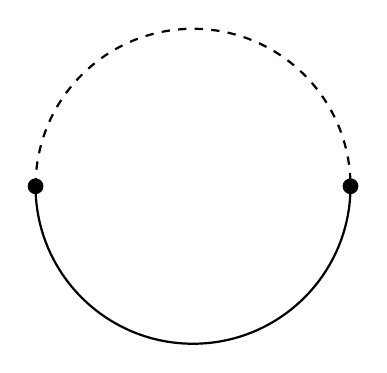
\begin{tikzpicture}
  \draw[thick] (0,2) arc(180:360:2);
  \draw[thick, dashed] (0,2) arc(180:0:2);
  \fill
    (0,2) circle (0.1)
    (4,2) circle (0.1)
  ;
\end{tikzpicture}
~~
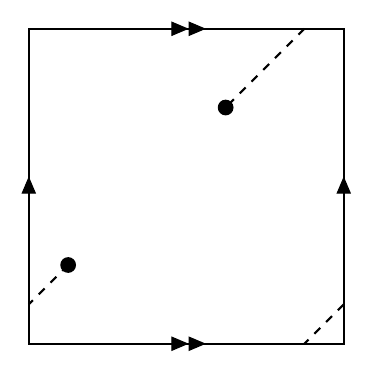
\begin{tikzpicture}
  \draw[thick] (0,0) rectangle (4,4);
  \draw[->>, >={triangle 45}] (0.25,0)--(2.25,0);
  \draw[->>, >={triangle 45}] (0.25,4)--(2.25,4);
  \draw[->, >={triangle 45}] (0,0.125)--(0,2.125);
  \draw[->, >={triangle 45}] (4,0.125)--(4,2.125);
  \fill
    (0.5,1) circle (0.1)
    (2.5,3) circle (0.1)
  ;
  \draw[thick, dashed]
    (0.5, 1)--(0,0.5) (4,0.5)--(3.5,0) (3.5,4)--(2.5, 3)
  ;
\end{tikzpicture}
    \caption{Illustrations of diameters on $S^1$ and $T^2$.}
  \end{figure}

  \begin{theorem}[Liokumovich, Nabutovsky, Rotman, 2014]
    % https://arxiv.org/abs/1410.8456
    Let $M$ be a Riemannian $2$-sphere. Then there exist three distinct simple
    geodesics with lengths that do not exceed $20d$ where $d$ is the diameter
    of $M$.
    Furthermore, if no simple closed geodesics of length $\leq 2d$, then there
    are three distinct simple periodic geodesics on M with lengths
    $\leq 5d$, $10d$, \text{ and } $20d$ respectively.
  \end{theorem}
  \begin{proof}[Proof idea]
    The above authors give their proof idea as follows: \begin{quote}
      The main idea of the proof of [the above theorem] is to express three homology
      classes of the space of non-parametrized curves that are used in classical
      proofs of the Lyusternik-Schnirelmann theorem by cycles that consist of
      simple closed curves ``mainly made'' of curves in a meridian-like family
      that connects two fixed points of $M$. [...] We attempt to construct such
      a family where the lengths of all meridians are bounded by const d for an
      appropriate const. Our repeated attempts can be blocked only by appearance
      of different “short” simple periodic geodesics of index 0. So, we either
      get three short simple periodic geodesics of index 0, or our third attempt
      to construct a “meridional slicing” succeeds. Once one of our attempts
      succeeds, and we get a slicing of $M$ into short meridians, the original
      proof of the Lyusternik-Schnirelmann theorem yields the desired upper
      bounds.
    \end{quote}
  \end{proof}
\end{section}

\end{document}
